\chapter{General}

\section{Installing an Operating System} \label{install_os}

To use the Raspberry Pi, an \gls{os} first needs to installed. \href{https://www.raspberrypi.org/downloads/raspbian/}{Raspbian Buster Lite} is the official \gls{os} for Raspberry Pi 4, and is used on every machine in the cluster.


After downloading the \gls{os}, uncompress the file. The extracted file should be of type \lstinline{.img}, containing a preinstalled Raspbian Buster \gls{os} that now must be written to the SD card. To write the image file to the SD card, several tools exists that can be used, with some examples as follows:

\begin{itemize}
    \item balenaEtcher (cross-platform)
    \item \lstinline{dd} (Linux)
\end{itemize}

Once the image has been successfully written, simply put the SD card into the Raspberry Pi machine and boot it. The default user that comes preinstalled is called \lstinline{pi}, with the default password \lstinline{raspberry}.


\section{Keyboard Layout} \label{keyboard_layout}

To change keyboard layout with a graphical user guide, simply run \lstinline{dpkg-reconfigure keyboard-configuration}. For most full-sized keyboards, the following options are what you want; \lstinline{Generic 105-key PC (intl.) -> Norwegian -> Norwegian -> The default for the keyboard layout -> No compose key}.


\section{Root Account} \label{root_account}

Once logged in with user \lstinline{pi}, create a root user with \lstinline{sudo passwd root}. Enter a chosen password. A root user has now been created. To use it, log out with \lstinline{logout} or simply reboot, and then log in as \lstinline{root}.

To delete the \lstinline{pi} user, issue the command \lstinline{deluser --remove-home pi} while logged in as \lstinline{root}.


\section{Updating the System} \label{update_system}

\textbf{Note:} \textit{If the current system is using a custom kernel, upgrading the system will also upgrade the kernel, thus overwriting the custom kernel. One can omit the \lstinline{upgrade} part if that is not desired.}

To update the system, run \lstinline{apt update && apt upgrade}. If an error about \lstinline{release file not valid yet} appears, the system's clock needs to be fixed. This can easily be done with the \lstinline{date} tool; \lstinline{date -s "15 Feb 2020 12:00"}.


\section{Enable SSH} \label{enable_ssh}

To enable SSH access, simply run \lstinline{systemctl enable ssh}. To allow SSH root login, the line \lstinline{PermitRootLogin yes} must be added to the file \lstinline{/etc/ssh/sshd_config}, which can conveniently be done with \lstinline{echo 'PermitRootLogin yes' >> /etc/ssh/sshd_config}. Then start SSH service with \lstinline{systemctl start ssh} or just reboot.


\section{Change Hostname} \label{change_hostname}

There are two files that needs to be edited in order to change hostname. First, the \lstinline{/etc/hostname} file, which only contains the current hostname. Simply change whatever is in it to what you want, say \lstinline{new_hostname}. Second, the file \lstinline{/etc/hosts} needs one line changed. Edit the line containg \lstinline{127.0.1.1} so that it looks as follows:

\begin{lstlisting}
127.0.1.1       new_hostname
\end{lstlisting}

Reboot to apply the changes.

% \section{Setting Up Dual Boot}

% First install Ubuntu. When asked for partitioning the disk, choose \lstinline{manual}, select the disk and confirm creating a new empty partition with \lstinline{yes}. Select the newly created empty partition followed by \lstinline{create a new partition} and set a size for it. The type should be of \lstinline{primary}, location at \lstinline{beginning} and mounting point \lstinline{root}. Finish off with \lstinline{done setting up the partition} followed by \lstinline{finish partitioning and write changes to disk}.

% % \begin{figure}[H]
% %     \centering
% %     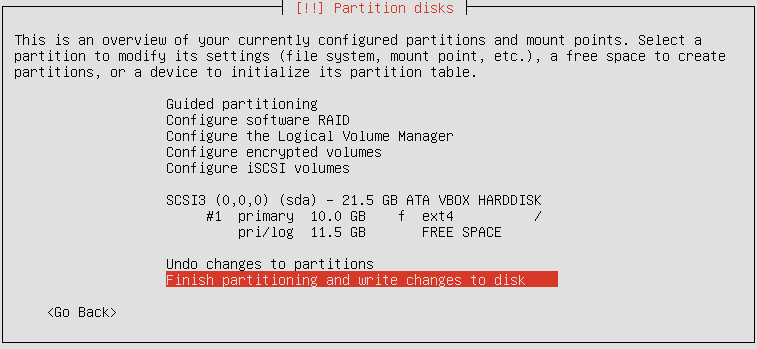
\includegraphics[width=0.75\linewidth]{ubuntu_partition}
% %     \captionsetup{width=0.75\linewidth}
% %     \caption{The partition editor for Ubuntu.}
% %     \label{fig:ubuntu_partition}
% % \end{figure}

% Next, install FreeBSD. When asked for partitioning the disk, choose \lstinline{auto (UFS)} followed by \lstinline{partition}. Set a size, hit \lstinline{ok} and \lstinline{finish}.

% % \begin{figure}[H]
% %     \centering
% %     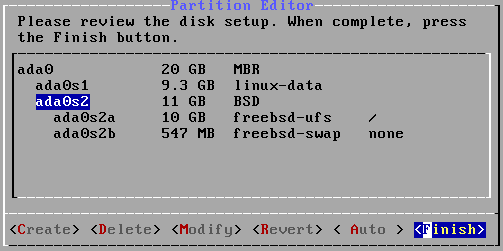
\includegraphics[width=0.75\linewidth]{freebsd_partition}
% %     \captionsetup{width=0.75\linewidth}
% %     \caption{The partition editor for FreeBSD.}
% %     \label{fig:freebsd_partition}
% % \end{figure}

% After installing both systems, only Ubuntu is presented in the \gls{grub}. To add FreeBSD as an option, run \lstinline{sudo nano /etc/grub.d/40_custom} in Ubuntu, and add the following entry:

% \begin{lstlisting}
% menuentry "FreeBSD" {
%     insmod ufs2
%     set root=(hd0,2)
%     kfreebsd /boot/loader
% }
% \end{lstlisting}

% Then update \gls{grub} with \lstinline{sudo update-grub}. The FreeBSD option should now be available when rebooting. If the bootloader won't display, hold the \lstinline{RIGHT SHIFT} key upon booting.

% To enable a one-time reboot into FreeBSD from Ubuntu, run the command \lstinline{grub-editenv /boot/grub/grubenv set next_entry="FreeBSD"} and reboot with \lstinline{sudo reboot}.





% \section{Compiling Mainline Kernel 5.5 for Raspberry Pi 4}


% \section{Patching web10g on Mainline Kernel 5.5}